\documentclass{article}
\pdfpagewidth=8.5in
\pdfpageheight=11in

\usepackage{ijcai26}
\usepackage{times}
\usepackage{url}
\usepackage[hidelinks]{hyperref}
\usepackage[utf8]{inputenc}
\usepackage[small]{caption}
\usepackage{graphicx}
\usepackage{amsmath}
\usepackage{booktabs}
\usepackage{array}
\usepackage[switch]{lineno}

% Comment out for camera-ready if requested by the venue.
\linenumbers
\urlstyle{same}

\hypersetup{
  pdfinfo={TemplateVersion={IJCAI.2026.0}}
}

\title{How Much Adaptation Is Enough?\\Drift Geometry and Minimal Calibration in Brain-to-Text BCI}

\author{Anonymous Authors}

\begin{document}
\maketitle

\begin{abstract}
Brain-to-text BCI decoders must remain usable as neural signals change across recording sessions. We audit how much input adaptation is needed when the official T15 brain-to-text GRU is evaluated across sessions. Native day-specific input layers reproduce low validation phoneme error (9.06\% PER), while forcing sessions through non-native input layers increases PER to 22.67--34.43\%. Unsupervised moment corrections fail to recover this loss. A supervised input-layer adapter trained from 20 labeled calibration trials improves the fixed-middle stress setting from 22.67\% to 18.59\% PER, but still leaves substantial degradation. The strongest practical result is source-layer selection: using a short unlabeled beginning-of-day window to choose a past input layer reaches 12.74\% PER at $K=20$, while the immediately previous session is even stronger at 12.21\%. Secondary geometry-only analyses show similar state structure beyond the main T15 decoder experiment. These results suggest that recency should be the default adaptation prior, while drift geometry is a useful signal for deciding when that default may need to be overridden.
\end{abstract}

\section{Introduction}
Do we really need to recalibrate or retrain a brain-to-text decoder every day? For a deployed BCI, this is a costly question: daily calibration takes user time, requires labeled data, and may still be unnecessary when a compatible input state already exists. Long-term stability has long been recognized as a central challenge for practical BCI deployment~\cite{vaadia2009grand}; here, ``drift'' means that the neural feature distribution recorded on a new day no longer matches the distribution seen by the decoder during earlier sessions. We show that the answer is not simply yes or no. In T15, the shared GRU decoder can remain frozen, but the input state must be chosen carefully: previous-session reuse is the strongest simple default, short-window geometry can retrieve older candidates, and labeled calibration is best treated as an escalation step rather than the first response.

We test this input-state view in the official T15 brain-to-text GRU baseline from a rapidly calibrating speech neuroprosthesis study~\cite{card2024accurate}. The model contains learned day-specific input layers, followed by a GRU and output head. Intuitively, each input layer acts like a small session-specific adapter that maps that day's neural features into the representation expected by the shared GRU decoder. This structure creates a useful stress test: if a target session is decoded through the wrong input layer, performance measures the decoder-facing cost of cross-session input mismatch. We then compare simple feature corrections, small learned adapters, and geometry-guided source selection as rungs of a lightweight adaptation ladder.

The contribution is not a new speech decoder. Instead, we provide a decoder-facing adaptation audit:
\begin{itemize}
    \item Wrong input states break the decoder: native-day PER is 9.06\%, while fixed non-native input layers increase PER to 22.67--34.43\%.
    \item Simple mean/scale correction is insufficient; input-layer calibration with $K=20$ improves PER to 18.59\% but remains far from native-day.
    \item Previous-session reuse is the strongest simple policy at $K=20$ (12.21\% PER), while geometry selection is close (12.74\%) and reveals older-state candidates.
    \item Geometry is a retrieval signal, not a standalone policy: at $K=20$ it selects older states in 11 sessions, but wins only 3 times, motivating a confidence gate.
\end{itemize}

We do not claim that neural drift geometry is new. Rather, we show that in a deployed-style brain-to-text decoder with learned day-specific input layers, short-window geometry is actionable for choosing among existing input-layer states and for framing recency as an explicit adaptation prior.

Figure~\ref{fig:conceptual-overview} summarizes this adaptation-ladder view: keep the shared decoder frozen, estimate the new input state from a short beginning-of-day window, and choose the lightest input-side action supported by the evidence.

\begin{figure*}[t]
\centering
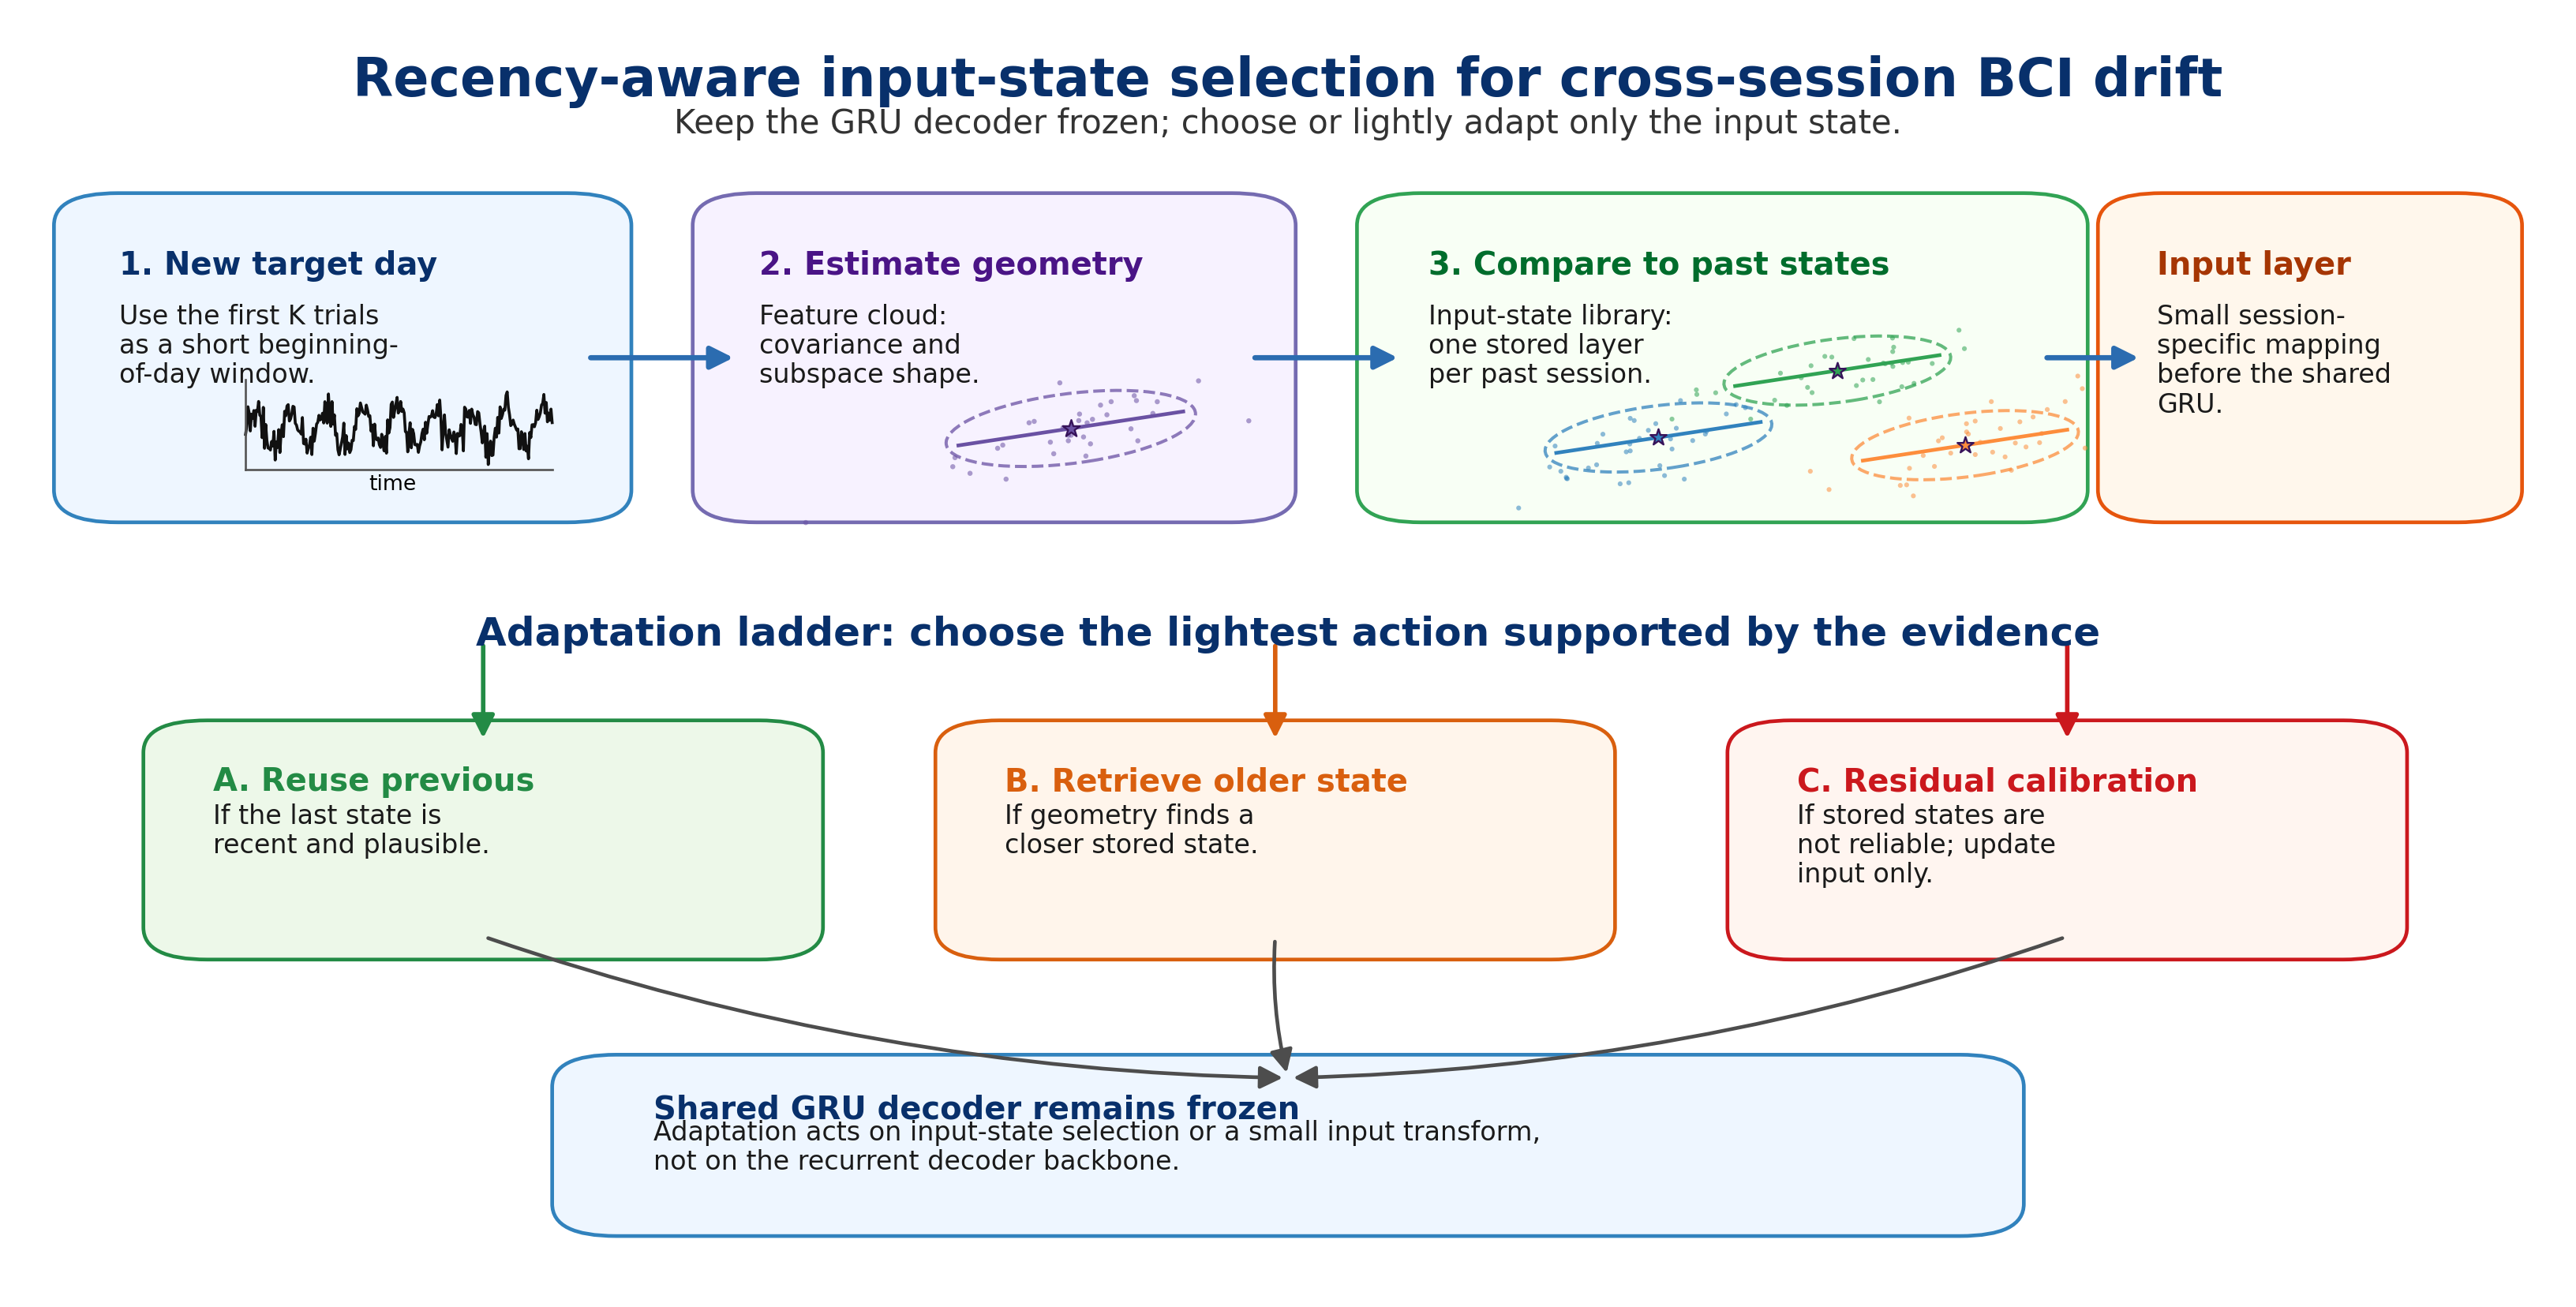
\includegraphics[width=0.88\textwidth]{figures/adaptation_ladder_overview.png}
\caption{Recency-aware adaptation ladder. A short beginning-of-day window estimates target-session geometry, compares it to stored input states, and chooses the lightest input-side action: reuse previous, retrieve an older candidate, or calibrate the input layer only. The GRU backbone and output head remain frozen.}
\label{fig:conceptual-overview}
\end{figure*}

\section{Related Work}
Brain-to-text BCIs have progressed from handwriting-based decoding to high-performance speech neuroprostheses, but long-term use still requires session-specific adaptation or recalibration as neural recordings change over time~\cite{willett2021handwriting,willett2023speech,card2024accurate}. Cross-session stability has also been studied through neural geometry and manifold alignment: prior work shows that low-dimensional neural structure can be aligned across recording instabilities, and dynamics-aware methods can stabilize BCIs over longer timescales~\cite{degenhart2020stabilization,karpowicz2025nomad}. Our setting is narrower: rather than learning a new invariant decoder, we ask whether short-window geometry can choose among existing day-specific input states. Continual recalibration and session-invariant learning provide complementary ways to update or regularize decoders~\cite{fan2023corp,zhang2026align}; here, we audit low-cost actions available before retraining: previous-session reuse, geometry-guided source retrieval, and lightweight input-layer calibration.

\section{Data and Decoder}
\textbf{T15.} The main experiments use 41 T15 validation sessions from the official brain-to-text copy-task dataset~\cite{card2024accurate}. Neural features are passed through the official GRU checkpoint and decoded greedily at the phoneme level. We compute phoneme error rate (PER) after standard CTC collapse; lower PER is better.

\textbf{Official baseline.} The decoder contains learned day-specific input layers, a shared GRU backbone, and an output layer over phoneme classes. Native-day decoding uses each session's own input layer. Cross-day stress tests use a fixed or selected non-native source input layer while keeping the GRU and output head unchanged.

\textbf{Beginning-of-day setting.} We use the first $K \in \{5,10,20\}$ trials of a target session for geometry estimation or supervised input calibration, and evaluate PER only on the remaining trials. T12 and inner-speech analyses are used only as geometry-only supporting checks, not decoder replications.

\section{Methods}
\subsection{Decoder-Facing Metrics}
For each T15 validation trial, we compute greedy phoneme predictions from the CTC output stream and apply CTC collapse before computing phoneme error rate. For a set of trials $\mathcal{D}$, the reported PER is
\[
    \mathrm{PER}(\mathcal{D}) =
    \frac{\sum_{i \in \mathcal{D}} \mathrm{edit}(y_i,\hat{y}_i)}
         {\sum_{i \in \mathcal{D}} |y_i|}.
\]
We avoid mixing PER with derived recovery percentages in the main result tables: lower PER is always better, and improvements are reported as direct PER changes.

\subsection{Adaptation and Source Selection}
We compare native-day decoding against three fixed non-native source layers: early (\texttt{t15.2023.08.13}), middle (\texttt{t15.2023.11.26}), and late (\texttt{t15.2025.04.13}). Using the middle source layer, we test a ladder of increasingly expensive input-side interventions: no correction, unsupervised mean/scale moment matching, supervised diagonal affine calibration, and supervised input-layer calibration. Moment methods test whether channel-wise distribution alignment is sufficient. Learned adapters use the first $K$ labeled trials and are evaluated on the remaining trials. The GRU backbone and output head remain frozen; only the input transform is learned using CTC loss.

\textbf{Neural feature geometry.} We represent each session as a cloud of neural feature vectors in channel space. Each time bin from each trial is one point in this space. The shape of this cloud is summarized using covariance and low-dimensional subspace statistics. For K-shot source selection, the first $K$ unlabeled target trials are used to estimate the target covariance. We then compare this covariance to each past source session using relative Frobenius covariance distance and reuse the input layer of the closest past session:
\[
    s^*(t) = \arg\min_{s \in \mathcal{S}_{\mathrm{past}}(t)}
    d_{\mathrm{cov}}(S_t^{(K)}, S_s).
\]
We compare this geometry policy to previous-session reuse, $s_{\mathrm{prev}}(t)$, because recency is the strongest prior available in a longitudinal BCI. We also compare bounded input-state libraries: previous only, last 3 sessions, last 5 sessions, and all past sessions.

\section{Experiments}
We first audit decoder-facing adaptation on T15, then use T12 and inner-speech blocks as geometry-only supporting checks.

Before presenting the detailed experiments, Table~\ref{tab:main-findings} summarizes the main empirical story. The results follow a simple adaptation ladder: wrong input states strongly degrade decoding, simple moment correction fails, small supervised calibration helps only partially, and the strongest low-cost intervention is to reuse or retrieve a compatible past input state.

\begin{table}[t]
\centering
\caption{Main findings at a glance. Lower PER is better.}
\scriptsize
\setlength{\tabcolsep}{3pt}
\begin{tabular}{@{}p{0.32\linewidth}p{0.26\linewidth}p{0.31\linewidth}@{}}
\toprule
Question & Result & Interpretation \\
\midrule
Does the native input state matter? & Native-day: 9.06\% PER & Correct day-specific input layers work well. \\
What if the input state is wrong? & Fixed non-native: 22.67--34.43\% PER & Cross-session mismatch strongly degrades decoding. \\
Is mean/scale correction enough? & Moment match: 22.73\% PER & Simple distribution matching fails. \\
Does small calibration solve it? & Input layer, $K=20$: 18.59\% PER & Calibration helps, but remains far from native-day. \\
What is the best low-cost policy? & Previous source, $K=20$: 12.21\% PER & Recency is the strongest default. \\
Does geometry help? & Geometry, $K=20$: 12.74\% PER; older wins 3/11 & Geometry retrieves candidates, but needs a gate. \\
\bottomrule
\end{tabular}
\label{tab:main-findings}
\end{table}

Thus, the central question becomes not whether adaptation is possible, but which input state should be used before any supervised calibration is attempted.

\subsection{Cross-Day Stress Test and Adaptation Ladder}
\textbf{Finding 1: the day-specific input layer is essential.}
Native-day decoding reaches 9.06\% phoneme-weighted PER, confirming that the local evaluation reproduces the expected behavior of the official checkpoint. When all sessions are forced through non-native source input layers, PER rises to 22.67--34.43\%, harming 40/41 sessions for each source choice.

\begin{table}[t]
\centering
\caption{T15 decoder-facing stress test and adaptation ladder. Mean, best-session, and worst-session values are phoneme-weighted PER. Fixed-source and moment-correction rows use the middle source \texttt{t15.2023.11.26}. Learned adapter rows use $K=20$ calibration trials and are evaluated on remaining trials. Lower PER is better.}
\scriptsize
\resizebox{\linewidth}{!}{%
\begin{tabular}{lccc}
\toprule
Condition & Mean PER $\downarrow$ & Best session & Worst session \\
\midrule
Native-day & 9.06\% & 0.80\% (11-19) & 23.82\% (03-14) \\
Fixed early & 28.81\% & 7.38\% (08-13) & 58.28\% (03-14) \\
Fixed middle & 22.67\% & 1.20\% (11-19) & 56.44\% (03-30) \\
Fixed late & 34.43\% & 16.40\% (01-12) & 49.04\% (07-19) \\
Moment match & 22.73\% & 1.20\% (11-19) & 56.90\% (03-30) \\
Diag. affine, $K=20$ & 20.21\% & 1.94\% (11-26) & 53.26\% (03-30) \\
Input layer, $K=20$ & 18.59\% & 2.46\% (11-26) & 52.23\% (03-30) \\
\bottomrule
\end{tabular}
}
\label{tab:ladder}
\end{table}

\begin{figure}[t]
\centering

\includegraphics[width=0.48\linewidth]{figures/t15_source_sweep_weighted_per.png}
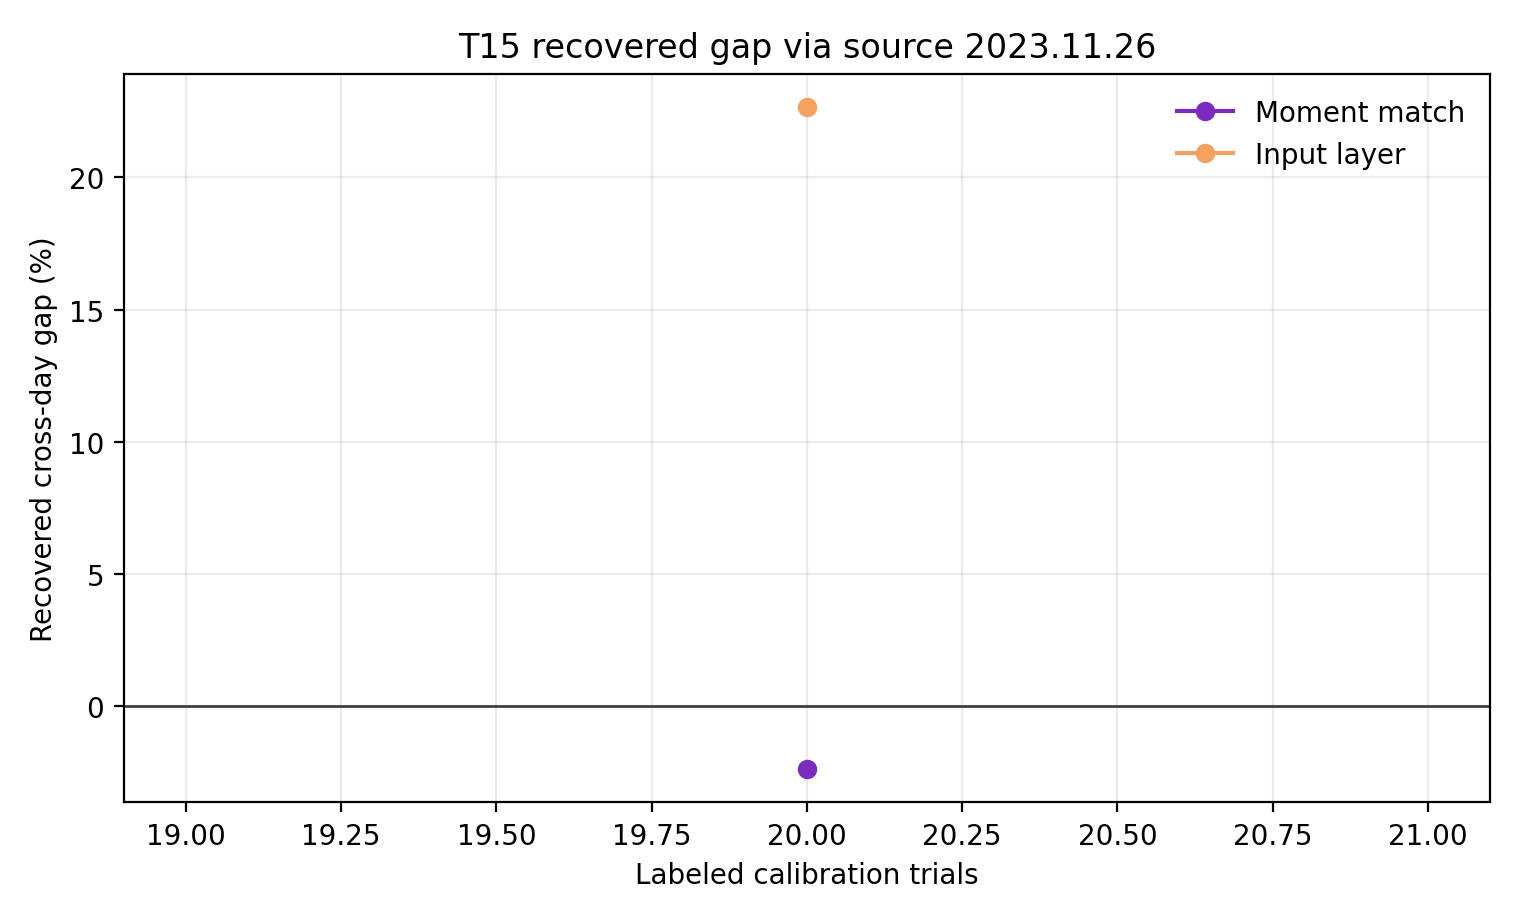
\includegraphics[width=0.48\linewidth]{figures/t15_input_layer_calibration_recovery_source_middle_K20_epochs20.png}
\caption{Left: fixed non-native source layers strongly degrade T15 phoneme decoding relative to native-day decoding. Right: small learned calibration improves over the fixed-middle source but remains far from native-day decoding.}
\label{fig:ladder}
\end{figure}

The natural first hypothesis is that cross-session mismatch is mostly a mean/variance shift. The data do not support this: moment matching remains essentially tied with no correction. Supervised diagonal affine and input-layer calibration improve PER beyond moment matching, with input-layer calibration reaching 18.59\% at $K=20$. However, this remains far from 9.06\% native-day decoding, so small calibration is useful but does not replace a well-matched prior input state.

\subsection{T15 Geometry and Beginning-of-Day Source Selection}
\textbf{Finding 2: T15 drift is geometrically structured over time.}
Before using geometry for retrieval, we first verify that T15 sessions have temporally structured input geometry. Figure~\ref{fig:t15-geometry-map} shows that pairwise covariance shift increases with temporal separation, while nearby sessions form a diagonal band of similar geometry. This supports recency as a strong prior, but the map is not purely chronological.

\begin{figure*}[t]
\centering
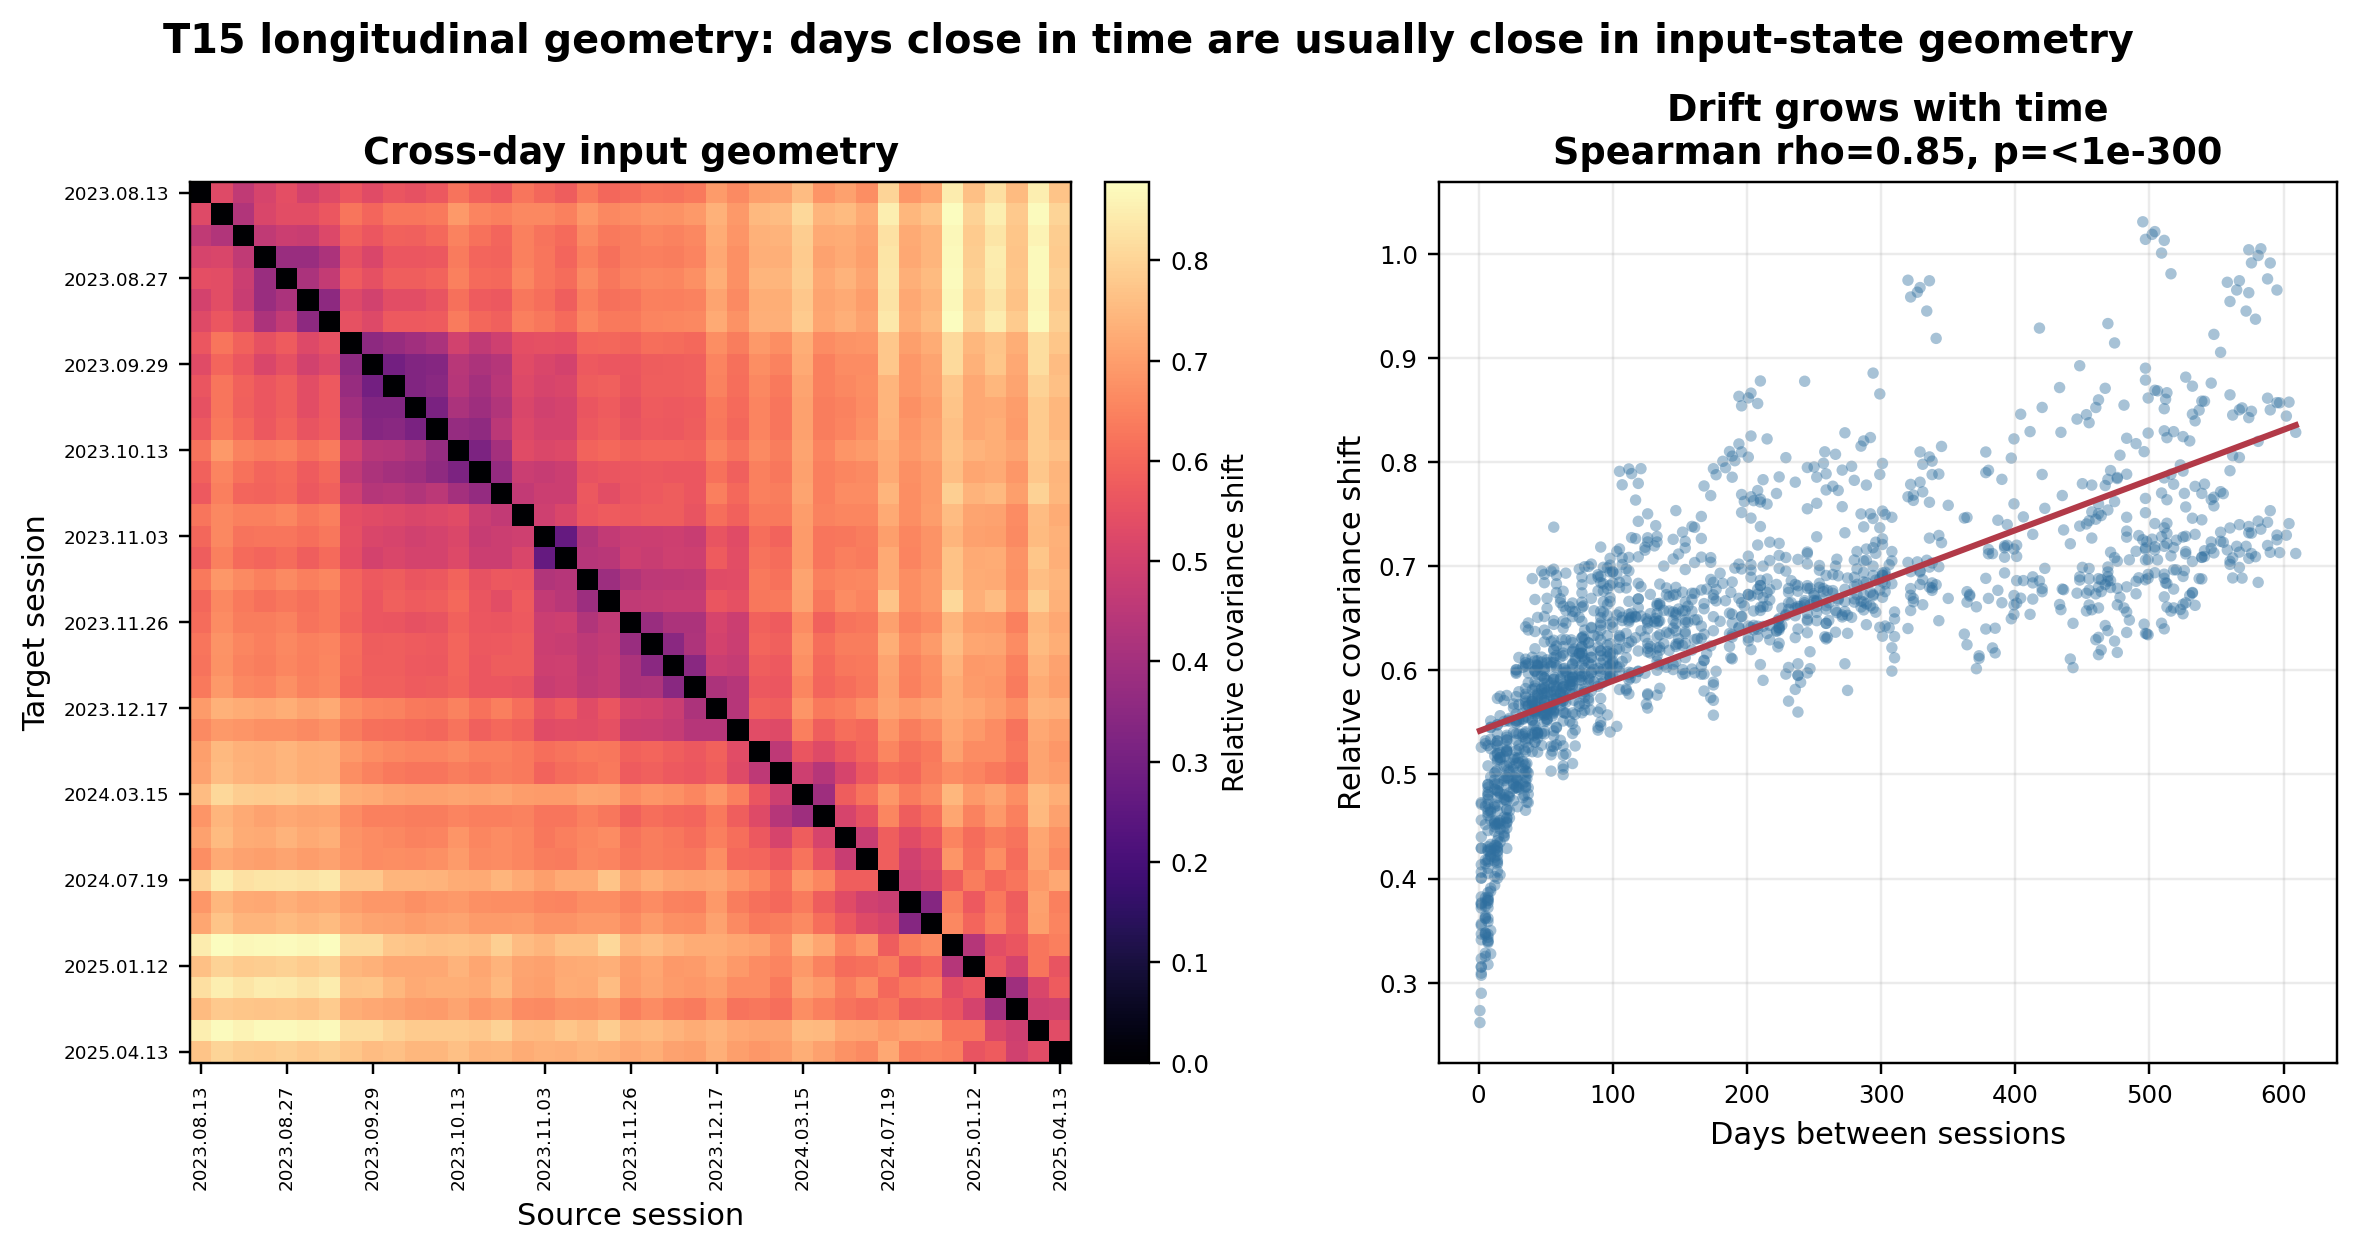
\includegraphics[width=\textwidth]{figures/t15_geometry_heatmap_scatter_covariance.png}
\caption{T15 longitudinal geometry map. Left: pairwise relative covariance shift between source and target sessions, ordered by date, shows a diagonal band of nearby sessions with similar input geometry. Right: covariance shift increases with temporal separation across source-target pairs (Spearman $\rho=0.85$), indicating that session geometry drifts with time while retaining non-monotonic structure.}
\label{fig:t15-geometry-map}
\end{figure*}

The beginning-of-day version is more realistic: the first $K$ trials estimate geometry or train a small adapter, and evaluation is performed only on the remaining trials. Past-only source selection reaches 14.00\%, 13.19\%, and 12.74\% PER at $K=5,10,20$, far below fixed-middle decoding on the same subsets. However, the immediately previous input layer is even stronger: 13.09\%, 12.84\%, and 12.21\% PER. This prior has a time horizon: previous-source PER is 9.97\% when the last available input state is 0--3 days old, 13.75\% at 4--14 days, and 24.54\% beyond two weeks. Thus previous is a strong default only when it is truly recent.

\begin{table}[t]
\centering
\caption{Beginning-of-day source selection on remaining validation trials. Previous-session recency is the strongest simple baseline, while K-shot geometry selection remains close and often selects non-previous sources. Lower PER is better.}
\small
\begin{tabular}{lccc}
\toprule
Method & $K=5$ & $K=10$ & $K=20$ \\
\midrule
Native-day & 8.95\% & 8.88\% & 8.90\% \\
Fixed middle & 22.51\% & 22.40\% & 22.30\% \\
Previous source & 13.09\% & 12.84\% & 12.21\% \\
K-shot geometry source & 14.00\% & 13.19\% & 12.74\% \\
Best simple override & 13.09\% & 12.90\% & 12.18\% \\
\bottomrule
\end{tabular}
\label{tab:kshot}
\end{table}

\subsection{Geometry Retrieves Older Candidates but Needs a Gate}
\textbf{Finding 3: geometry retrieves older candidates, but does not reliably replace recency.}
The previous-session input layer is the strongest simple baseline, but it is not always the geometrically nearest source. At $K=20$, geometry selects the previous source in 26 sessions and an older non-previous source in 11 sessions. Among those 11 older selections, the older source achieves lower PER in 3 cases, the previous source remains better in 7 cases, and 1 case is tied. Thus geometry identifies plausible older-state candidates, but covariance distance alone is not sufficient as a deployment policy: closer in geometry does not always mean lower PER.

\begin{figure}[t]
\centering
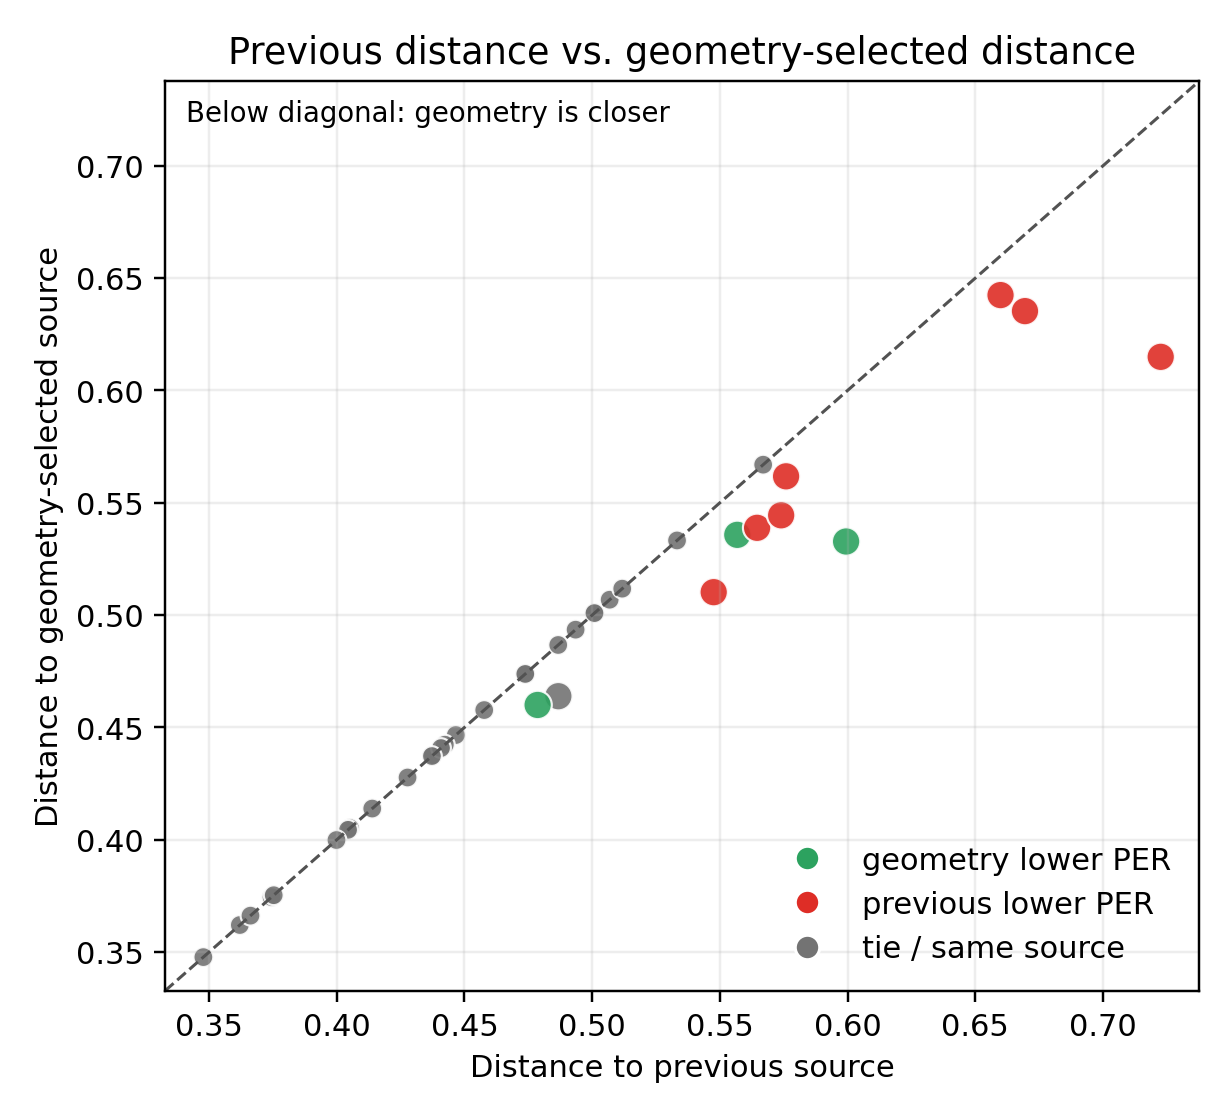
\includegraphics[width=\linewidth]{figures/t15_geometry_previous_vs_selected_distance.png}
\caption{Geometry retrieves closer candidates but is not a standalone policy. Points below the diagonal have a geometry-selected source that is closer than the previous source in covariance distance. Green points indicate cases where the geometry-selected source achieves lower PER; red points indicate cases where previous remains better.}
\label{fig:geometry-nonprevious-story}
\end{figure}

This motivates retaining a compact memory of input states rather than only the latest layer. We restrict K-shot geometry selection to previous only, the last 3 sessions, the last 5 sessions, or all past sessions. The immediately previous session remains the best aggregate policy, but a small recent library nearly matches all-past selection.

\begin{table}[t]
\centering
\caption{K-shot input-state library-size ablation. PER is measured on remaining validation trials after using the first $K$ trials to estimate target geometry. A bounded recent library nearly matches all-past selection, while previous-only recency remains the strongest aggregate baseline.}
\small
\begin{tabular}{lcccc}
\toprule
$K$ & Previous & Last 3 & Last 5 & All past \\
\midrule
5 & 13.09\% & 13.47\% & 13.55\% & 14.00\% \\
10 & 12.84\% & 13.19\% & 13.19\% & 13.19\% \\
20 & 12.21\% & 12.76\% & 12.74\% & 12.74\% \\
\bottomrule
\end{tabular}
\label{tab:library-size}
\end{table}

A simple distance-ratio gate does not yet solve this problem. At $K=20$, the best simple override improves only marginally from 12.21\% to 12.18\% PER, and a leave-one-session-out decision stump improves only to 12.15\% while performing worse at smaller $K$. Older sources beat previous in only a minority of non-previous selections (3/11, 4/9, and 3/11 for $K=5,10,20$), so future gates need richer confidence features.

To ask why older sources sometimes help, we compare drift fingerprints for target--previous and target--older-source pairs. Although older-source wins are rare, they are better explained by subspace geometry than by mean/scale shifts alone. When older sources win, they reduce the mean principal angle relative to previous by 1.37$^\circ$, 1.93$^\circ$, and 2.91$^\circ$ for $K=5,10,20$; when older sources lose, this subspace improvement is absent or reverses.

\begin{table}[t]
\centering
\caption{Preliminary drift fingerprints for non-previous source choices. Negative principal-angle change means the older source is closer to the target subspace than the previous source.}
\small
\begin{tabular}{lccc}
\toprule
$K$ & Case & $n$ & $\Delta$ principal angle \\
\midrule
5 & older wins & 3 & -1.37$^\circ$ \\
5 & older loses & 8 & -0.06$^\circ$ \\
10 & older wins & 4 & -1.93$^\circ$ \\
10 & older loses & 5 & +1.02$^\circ$ \\
20 & older wins & 3 & -2.91$^\circ$ \\
20 & older loses & 8 & +0.55$^\circ$ \\
\bottomrule
\end{tabular}
\label{tab:drift-fingerprints}
\end{table}

\subsection{Geometry-Only Supporting Checks}
T12 diagnostic blocks provide a secondary geometry-only check. Across spike-power and threshold-crossing feature variants, covariance distance increases with temporal separation, and geometry sometimes selects older non-previous sessions. For spike-power features, geometry selects an older source in 7/15 targets, including a 53-day non-recent match.

As a separate behavior-state check, we analyzed inner-speech behavior blocks without training a decoder or attempting inner-speech decoding. Covariance geometry retrieves matching behavior well above chance, with binned threshold crossings during the go epoch reaching 96.15\% nearest-behavior accuracy versus a 20\% chance level. These results support the broader input-state view, but remain geometry-only.

\section{Discussion}
The main lesson is that cross-session adaptation should not be treated as a single fixed correction. Native T15 input layers are highly effective, while fixed non-native input layers cause large decoder-facing degradation. Simple moment alignment does not emulate those layers, and learned input calibration improves PER only partially. The most useful low-cost intervention is therefore not a new adapter, but a better choice of existing input layer.

A small number of difficult sessions, especially 2025-03-30 and 2025-03-14, dominate worst-case PER. However, sensitivity checks excluding the worst one or two sessions preserve the same qualitative ordering: fixed non-native layers remain degraded, moment matching remains ineffective, input-layer calibration remains partial, and previous/geometry source policies remain the strongest low-cost choices. We therefore retain all sessions and treat these days as stress cases for future session-quality gating.

The practical policy is a beginning-of-day triage. The system should first reuse the previous input state, because it is the strongest simple default when truly recent. If short-window geometry suggests that the new session resembles an older stored state, the system can retrieve that state from a compact library. If no stored state appears reliable and labels are available, residual calibration can update only the input transform while leaving the GRU backbone and output head frozen.

Geometry should not be treated as a replacement for recency. At $K=20$, it identifies older non-previous candidates in 11 sessions, but those candidates beat previous in only 3 cases. The drift-fingerprint analysis suggests that subspace mismatch is more informative than covariance distance alone when deciding whether an older state is worth retrieving. Future gates should combine subspace features, distance margins, temporal gap, decoder confidence, and session-quality diagnostics.

This framing complements stronger decoder-backbone approaches. Pretrained speech models or language-model decoding may improve absolute performance, while input-state selection addresses a different deployment question: how to keep a fixed decoder usable across sessions with minimal calibration. Future work should test this ladder with WER, language-model decoding, closed-loop evaluation, and additional datasets. Preliminary alignment probes also suggest caution: geometry-based feature transformations such as covariance alignment may introduce harms, so geometry is currently more reliable as a retrieval signal than as an automatic feature transformation.

\section{Limitations}
This study is a decoder-facing audit, not a new decoding architecture. We report greedy phoneme error rate rather than full WER or language-model decoding. T12 and inner-speech analyses are geometry-only and should not be interpreted as decoder replications. The learned-adapter and K-shot source-selection experiments simulate a beginning-of-day window within the validation split and evaluate only on remaining trials. Larger windows can be informative, but we focus on $K \leq 20$ as the minimal-calibration regime.

\section{Conclusion}
For T15 brain-to-text decoding, fixed non-native input layers break the decoder, moment correction is too weak, and learned input adaptation improves PER only partially. The largest practical improvement comes from selecting a compatible past input layer. The immediately previous session is a strong default, while drift geometry is a measurable signal for deciding when that default may need to be overridden. This supports a recency-aware, geometry-guided adaptation ladder: start with the previous input state, measure drift geometry from a short unlabeled window, and move to stronger calibration only when the geometry indicates that simple source selection is not enough.

\section*{Ethical Statement}
This work uses publicly released intracortical BCI datasets and reports only aggregate analyses. It does not attempt to infer private inner speech or deploy a decoder. Future extensions to inner-speech or cross-behavior state selection should include explicit intent-gating and privacy safeguards.

\clearpage
\bibliographystyle{named}
\bibliography{ijcai26}

\end{document}
